% Session 4 -- the Laughlin quasihole: a depletion of fractional charge, and the
% Berry phase that measures both its charge and its exchange statistics.
% Placement: sec. "Berry phase, fractional charge, and anyonic statistics",
% after equation (4.16).
% Rendered by figures/blender/s04f06_quasihole.py, labels in figures/overlays/s04f06_quasihole.tex.
\begin{aqmfigure}{fig:s04:quasihole}{Fractional charge and fractional statistics, both obtained from
a Berry phase. (a) When we multiply the Laughlin state by $\prod_i(z_i-w)$, equation (4.14), the
angular momentum of every electron about $w$ increases by one, which by figure~\ref{fig:s04:droplet}
moves charge radially outward and leaves a region with less charge behind, the dimple. If we do this
$m$ times we remove exactly the charge of one electron, so one quasihole has the charge of an
electron divided by $m$, which is $q=e/m$. (b) When we move one quasihole once around another, along
the loop, and follow the Berry phase, it separates into two parts. The first is an Aharonov-Bohm
part, proportional to the enclosed flux, and its prefactor is what fixes $q=e/m$ in (4.15). The
second is a remaining part $2\pi/m$, which depends only on the fact that one quasiparticle went
around the other. A full loop is two exchanges, so the exchange phase itself is $\pi/m$, drawn at
the bottom for $m=3$. For every odd $m>1$ it is strictly between the bosonic $0$ and the fermionic
$\pi$, and this is what makes these excitations anyons.}
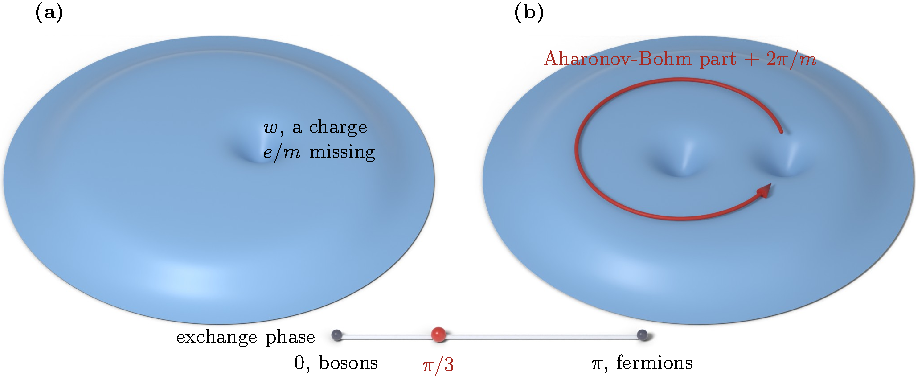
\includegraphics{figures/pdf/s04f06_quasihole.pdf}
\end{aqmfigure}
